\documentclass[11pt,a4paper]{article}

\usepackage{kotex}
\usepackage[margin=1in]{geometry}
\usepackage{graphicx}
\usepackage{booktabs}
\usepackage{hyperref}
\usepackage{amsmath}
\usepackage{amssymb}
\usepackage{xcolor}
\usepackage{listings}
\usepackage{microtype}
\usepackage{url}
\usepackage{enumitem}
\usepackage{float}

\setlength{\parskip}{0.3em}
\setlength{\parindent}{0pt}

\hypersetup{
  colorlinks=true,
  linkcolor=blue!60!black,
  urlcolor=blue!60!black,
  citecolor=blue!60!black,
}

\lstset{
  basicstyle=\ttfamily\small,
  breaklines=true,
  frame=single,
  framesep=4pt,
}

\title{\textbf{nature}: LLM 에이전트 시스템의\\
       체계적 실험을 위한 플랫폼}
\author{Chanhyeok Kim\thanks{\texttt{chanhyeok\_kim@icloud.com}}}
\date{\today}

\begin{document}
\maketitle

\begin{abstract}
LLM 에이전트 시스템은 이제 연구 데모가 아닌 프로덕션 현실이며, 그
동작은 여러 설계 선택의 상호작용에 의존한다: 모델, 프롬프트, 도구
권한, 위임 토폴로지, 메모리 압축, 어댑터 스택, aggregator 라우트.
설정을 고정하고 모델만 바꾸는 벤치마크는 유용한 한 가지 이야기를
들려줄 뿐 전체 이야기가 아니다. 본 논문은 \textbf{nature}를 제시한다
\textemdash\ 각 설정 축을 swappable한 파일 기반 아티팩트로 만들고,
모든 실행을 event-sourced 로그로 남겨 재생/counterfactual fork/사후
분석이 가능한 플랫폼이다. 세 가지 예시 연구가 이 프리미티브들이
무엇을 가능케 하는지 보여준다: 5-preset $\times$ 5-task 종단 벤치마크는
동일 모델 계열 내에서 2.3$\times$ 비용 분산 (preset별 평균 max/min)과 receptionist $\times$
downstream-model 상호작용 효과를 드러내고; 13개 로컬 + 11개 클라우드
모델에 걸친 구성요소 수준 probe sweep은 provider-family 정성적 특질과
측정 artifact를 발견하며 (4개 로컬 모델이 처음엔 잘못 채점됨; 1개
클라우드 모델은 aggregator 라우팅 계층 때문에 사용 불가);
event-pinned counterfactual fork는 swap-and-run 실험이 구조적으로
제공할 수 없는 "post-fork metric delta를 단일 변수에 깨끗이
귀속시키는" 프리미티브를 증명한다. 30-fork 페어드 분석은 open-ended
코드 분석 followup에서 Jaccard CI를 1.38$\times$ 타이트하게 만들고
($z=3.19$), 세 가지 followup 계열에 걸쳐 효과의 prompt-regime 의존성을
특성화한다 \textemdash\ open-ended 분석 regime에서는 깨끗하게
작동하나 제약된 사실 또는 다양성 추구 regime에서는 그렇지 않다.
플랫폼은 오픈소스이며 \url{https://github.com/chanhyeok-made/nature-platform}
에서 확인 가능.
\end{abstract}

\section{서론}

LLM 에이전트 시스템은 짧은 기간 안에 연구 데모에서 프로덕션 도구로
이동했다. 이를 배포하는 팀은 세션당 수십 가지 설정 결정을 내린다:
어떤 모델이 어떤 역할을 맡는가, 위임 토폴로지를 어떻게 배선하는가,
각 역할이 어떤 도구를 호출할 수 있는가, 메모리를 어떻게 압축하는가,
어떤 aggregator가 호출을 라우팅하는가, 실패는 어떻게 재시도하는가.
모든 축이 모든 다른 축과 상호작용한다. 연구자 역할 선택 (예: 로컬
phi4:14b vs 클라우드 haiku-4.5)은 모델 비교가 아니다 \textemdash\
그것은 비용/지연 프론티어를 단일 모델 벤치마크가 감지할 수 없는
방식으로 이동시키는 멀티호스트 라우팅 결정이다.

이 분야의 진전은 각 변수를 분리, 교체, 측정할 수 있는 플랫폼을
필요로 한다 \textemdash\ 단순한 애플리케이션 프레임워크도, 정적
벤치마크도 아닌. \textbf{nature}는 그러한 플랫폼의 한 가지 구현이다.
기여:

\begin{enumerate}[leftmargin=*,itemsep=2pt,topsep=2pt]
\item 각 설정 축을 일급(first-class)이며, composable하고 파일 기반인
      아티팩트로 취급하는 아키텍처 (Pack, Host, Agent, Preset).
\item 모든 실행을 재현/사후 분석 가능하게 만들고, \emph{독특하게}
      event-pinned counterfactual을 지원하는 event-sourced 실행:
      기록된 세션을 임의의 결정 시점에서 fork하여, 변형된 설정
      아래에서 이어서 실행하고, 그 결과로 나타나는 delta를 post-fork
      변수에 깨끗이 귀속시킨다.
\item 예시 연구 \textemdash\ 5-preset 벤치마크 (\S\ref{sec:preset-benchmark}),
      24-모델 probe sweep (\S\ref{sec:probes}), 두 가지 event-pinned
      ablation (\S\ref{sec:ablations}) \textemdash\ 은 플랫폼이 실제로
      사용되는 모습과 단일 모델 벤치마킹이 놓치는 발견들을 보여준다.
\end{enumerate}

\section{관련 연구}

각 시스템이 무엇을 최적화하는지에 따라 분류한다.

\textbf{애플리케이션 프레임워크.} LangChain, LlamaIndex, CrewAI,
AutoGen은 \emph{앱 구축}에 최적화되어 있다 \textemdash\ 주요 ergonomics
타겟은 에이전트 구성과 배포이며, 설정 축에 걸친 체계적 변이가
아니다. nature는 상호보완적이다: 파일 기반 축 분해는 이들 프레임워크가
직접 노출하지 않는 방식으로 각 차원을 독립적으로 swappable하게 만든다.

\textbf{프로덕션 모니터링 / 평가.} LangSmith, Arize, Weights \& Biases
(prompts)는 라이브 trace와 파이프라인 수준 eval에 집중한다. 요청당
데이터를 드러내지만 분리-변수 실험을 겨냥하지 않는다: 두 프롬프트를
비교하는 연구자는 프로덕션 trace 두 개(로드 밸런싱 라우팅 +
temperature로 교란됨)를 돌리거나 별도 오프라인 harness를 세팅해야 한다.

\textbf{정적 벤치마크.} SWE-bench, AgentBench, HumanEval, MLE-bench는
고정 태스크 세트에서 모델을 비교한다. 설계상 모델 축이 고정되어 있다
\textemdash\ 모델 주변의 설정은 전제된다. \S\ref{sec:preset-benchmark}의
preset 벤치마크는 그 "전제된" 공간이 실제로 얼마만큼 metric을 움직이는지
보여준다.

\textbf{실험 추적 (ML).} MLflow, W\&B는 파라미터와 메트릭을 추적하지만
모델 수준이며 에이전트 토폴로지를 인지하지 못한다. Event-sourced fork는
이들 중 어디에도 프리미티브로 존재하지 않는다.

\textbf{인접: MCP / 도구 생태계.} MCP 스펙은 도구-모델 인터페이스를
표준화하지만 설정 위 실험을 다루지 않는다. nature는 그 위에 놓인다
\textemdash\ MCP가 도구를 공급하면 nature가 에이전트의 도구 사용 방식을
둘러싼 실험 harness를 공급한다.

Gap: \emph{LLM 에이전트 시스템의 모든 축에 걸친 composable하고 파일
기반이며 재현 가능한 실험}. nature가 차지하는 niche다.
Table~\ref{tab:related-comparison}이 이 gap을 7개 구체적 실험-시점
역량으로 매핑하고 각 카테고리 대표 시스템에 대해 표시한다.

\begin{table}[H]
\centering\footnotesize
\setlength{\tabcolsep}{4pt}
\resizebox{\textwidth}{!}{%
\begin{tabular}{l c c c c c c c}
\toprule
실험-시점 역량 & LangChain & LangGraph & AutoGen & CrewAI & LangSmith & MLflow/W\&B & nature \\
\midrule
역할별 모델 swap (단일 edit)                & $\circ$ & $\circ$ & $\circ$ & $\circ$ & ---     & ---     & $\bullet$ \\
역할별 prompt / tool-permission swap        & $\circ$ & $\circ$ & $\circ$ & $\circ$ & ---     & ---     & $\bullet$ \\
행동 intervention을 composable artifact로  & ---     & ---     & ---     & ---     & ---     & ---     & $\bullet$ \\
세션 로그로부터 deterministic replay        & ---     & $\circ$ & ---     & ---     & $\circ$ & ---     & $\bullet$ \\
실행 도중 fork + config mutation            & ---     & $\circ$ & ---     & ---     & ---     & ---     & $\bullet$ \\
로그로부터 사후 metric 추출                 & ---     & ---     & ---     & ---     & $\bullet$ & $\circ$ & $\bullet$ \\
구성요소 수준의 분리된 capability probe     & ---     & ---     & ---     & ---     & ---     & ---     & $\bullet$ \\
\bottomrule
\end{tabular}}
\caption{대표 시스템 별 실험-시점 역량. 각 표시는 본 글 작성 시점
기준 documented된 시스템 capability를 반영하며, 충분한 custom
code로 가능한 범위가 아니다. $\bullet$ = repository-native하고
documented되었으며 first-class 실험 프리미티브로 노출됨 (예: 단일
declarative config edit 또는 명명된 API 한 번). $\circ$ =
실험별 custom code (subclassing, 수동 checkpoint plumbing,
callback wiring)로 달성 가능하나 first-class 프리미티브로
노출되지 않음. --- = documented 또는 practical 경로 알려지지 않음.
근거: LangChain~\cite{langchain}, LangGraph~\cite{langgraph},
AutoGen~\cite{autogen}, CrewAI~\cite{crewai},
LangSmith~\cite{langsmith}, MLflow~\cite{mlflow},
W\&B~\cite{wandb}; LlamaIndex~\cite{llamaindex}는 주축 (데이터
ingestion / retrieval)이 본 실험-축 비교 밖에 있어 표에서 제외.
표에서 가장 load-bearing한 $\circ$는 LangGraph의 checkpoint
프리미티브이다: 이전 상태로의 rewind는 지원하지만, resume-under-
mutated-configuration (\S\ref{sec:primitives}이 nature를 위해
formalize한 연산)은 본 글 작성 시점 기준 documented LangGraph
프리미티브가 아니다. LangSmith의 metric extraction $\bullet$은
trace-based evaluation API를 반영; replay $\circ$는 변형된 설정
하의 deterministic re-execution은 없는 trace-inspection 지원을
반영.}
\label{tab:related-comparison}
\end{table}

\section{아키텍처}
\label{sec:architecture}

nature의 아키텍처는 에이전트 시스템을 6개 계층 아티팩트로 분해하며,
본 논문의 사례 연구들은 각 계층을 분리된 실험 축으로 변화시킨다. 이
분해는 의도적으로 파일 기반이다: 기여자는 새 Pack, Agent, 또는 Preset을
`.json' (스키마 검증됨)과 선택적 `.md' (역할 지시서) 쌍으로 작성하여
저장소에 커밋하기만 하면, 이후 모든 실행이 이름으로 참조할 수 있다.
학습해야 할 스크립팅 API도 없고, 부트스트랩해야 할 레지스트리도 없다.

\textbf{Pack} \textemdash\ 개입(Gate / Listener / Contributor)을 파일 기반
discoverable 단위로 묶은 것. Gate는 도구 호출을 가로채 입력을 변형하거나
합성 결과로 단락 회로하거나 거부할 수 있다. Listener는 프레임 생애주기와
LLM span 이벤트를 수동적으로 관찰한다. Contributor는 나가는 LLM 요청에
보조 콘텐츠를 주입한다. Pack은 \emph{동작 정책}을 swappable 변수로
분리한다: "프레임당 비싼 도구 호출 rate-limit" 같은 변경은 에이전트
loop을 관통하는 diff가 아니라 단일 Pack 파일이다.

\textbf{Host} \textemdash\ 모델 엔드포인트(HTTP base URL + API 키 env var +
provider 어댑터) + 모델 카탈로그. 이를 사용하는 역할로부터 분리되어,
Preset이 역할 정의를 편집하지 않고도 동일 역할을
\texttt{local-ollama::phi4:14b}에서 \texttt{anthropic::claude-haiku-4-5}로
재라우팅할 수 있다. Host는 \emph{모델 선택}을 swappable 변수로 분리한다.

\textbf{Agent} \textemdash\ 역할 정의(JSON 셸 + .md 지시서 본문). JSON은
허용된 도구, 모델 참조, 역할 설명을 선언한다; .md는 프롬프트를 담는다.
\emph{프롬프트 / 도구 권한 / 역할 계약}을 swappable 변수로 분리한다.
\texttt{researcher-scout}(경로만) 같은 역할 변형은 JSON을 공유하고 .md만
다르게 하여 \S\ref{sec:ablations}의 프롬프트 ablation을 가능케 한다.

\textbf{Preset} \textemdash\ Agent를 팀으로 선언적으로 조합한 것:
`root\_agent', 도달 가능한 서브에이전트 명단, `model\_overrides' (역할별
Host::model), `prompt\_overrides' (역할별 지시서 stem 교체). Preset 파일은
\S\ref{sec:preset-benchmark}에서 전체 설정을 비교하는 단위다.

\textbf{Event-sourced frames} \textemdash\ 모든 결정은 세션당 JSONL 이벤트
로그에 append된다. 프레임 생애주기, LLM 요청/응답, 도구 시작/완료, 위임
경계, 압축 이벤트가 모두 이벤트다. 재생은 결정적이다:
\texttt{reconstruct()}는 LLM을 다시 호출하지 않고도 임의의 과거 프레임
트리를 로그로부터 재구성한다. 메트릭(비용, 지연, 턴 수, 도구 에러 수,
서브프레임 깊이)은 런타임에서 캡처되지 않고 사후에 로그에서 추출된다.
이것이 event-pinned counterfactual fork를 가능케 한다: 브랜치는 이벤트
$N$까지의 prefix 로그를 복사하고 $N{+}1$부터 새 설정 아래에서 이어간다.

\textbf{Memory compaction pipeline} \textemdash\
\texttt{BodyCompactionPipeline}은 모델별 컨텍스트 예산에 따라 모든 LLM
호출 전에 실행된다. 전략(\texttt{MicrocompactBodyStrategy}는 오래된
tool-result를 축출; \texttt{DreamerBodyStrategy}는 요약하고 원본 slice를
세션 스코프 long-term-memory 디렉터리에 보존)은 swappable
\texttt{BodyCompactionStrategy} 인스턴스다. 모든 압축은
\texttt{BODY\_COMPACTED} 이벤트를 emit하며 payload는 post-compaction body
스냅샷이므로 재생은 byte-identical이다. \emph{컨텍스트 압축 정책}을
swappable 변수로 분리한다.

6개 계층은 세션 생성 시 조합된다: Preset은 Agent를 참조하고, Agent는
Host를 참조한다; Pack은 area manager에 설치된다; Composer는 모든 LLM
호출 전에 압축 파이프라인을 참조한다. 어느 한 계층을 교체하는 기여자는
다른 계층을 건드리지 않는다. Figure~\ref{fig:architecture}가 compose-and-
dispatch 관계를 요약한다.

\begin{figure}[H]
  \centering
  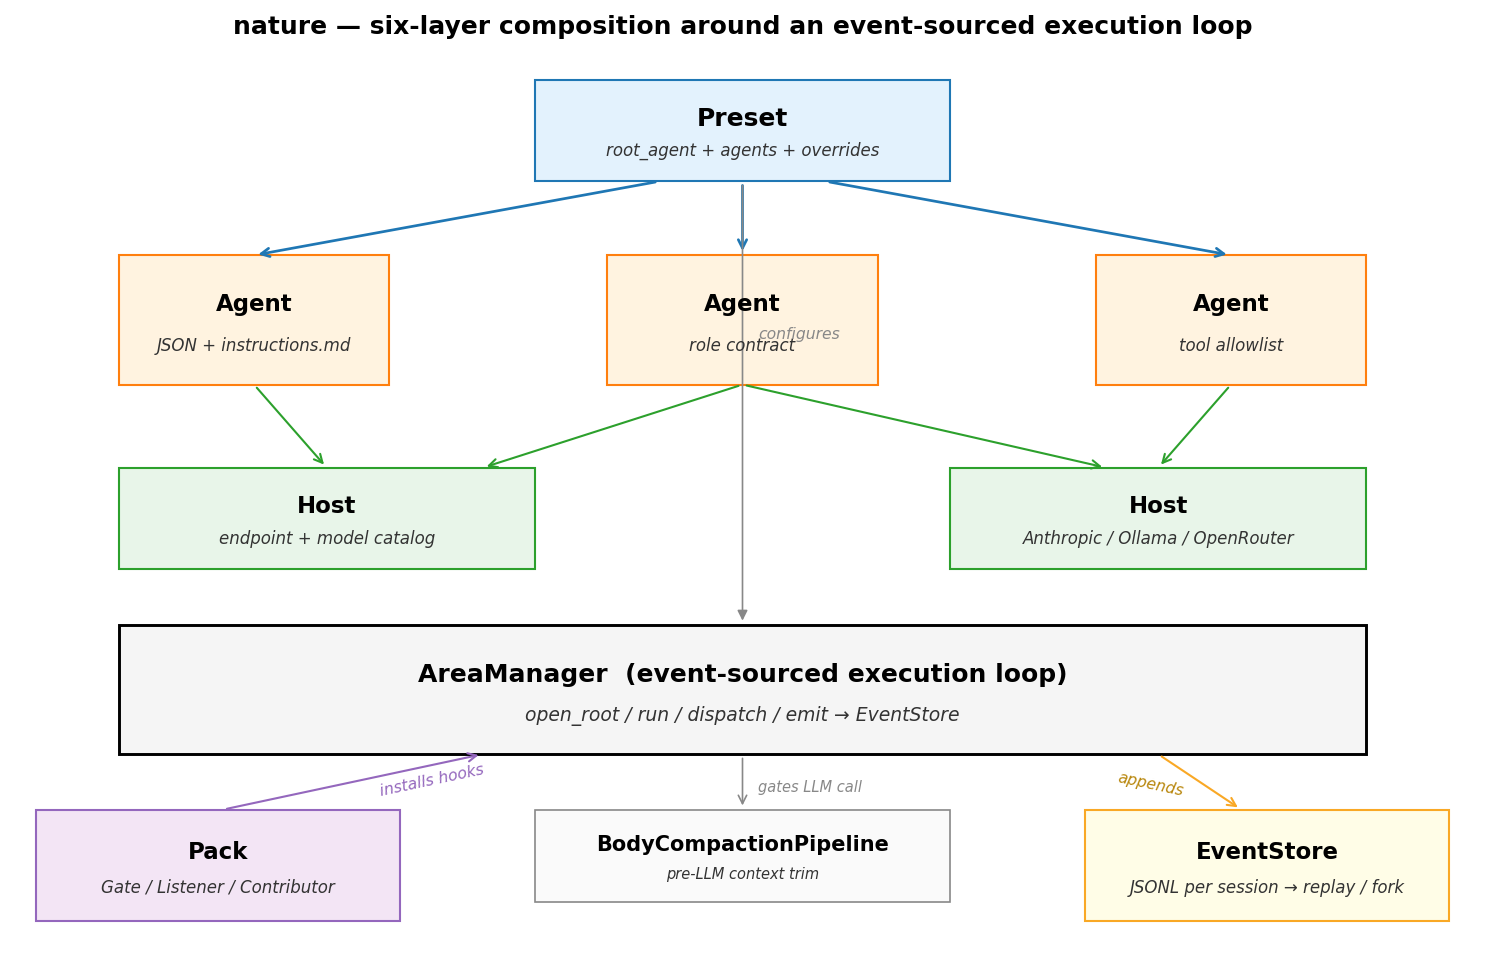
\includegraphics[width=0.95\textwidth]{figures/fig_architecture.png}
  \caption{nature의 6계층 아키텍처. Preset이 Agent를 선택하고 파라미터화하며,
           각 Agent는 모델을 해석하는 Host를 가리키고, AreaManager가 결과
           실행 loop을 dispatch하면서 모든 결정을 세션 EventStore에 append
           한다. Pack은 manager에 hook을 설치하고, BodyCompactionPipeline은
           나가는 모든 LLM 호출을 gate한다. 계층 간 모든 edge는 하드코드된
           의존이 아니라 파일 기반 아티팩트 참조다.}
  \label{fig:architecture}
\end{figure}

\section{실험 프리미티브}
\label{sec:primitives}

\textbf{Swap-and-run.} Pack / Host / Agent / Preset 하나를 교체하고 처음부터
재실행. 저렴하지만 per-run 분산(샘플링, 도구 상태, 외부 호출 순서)이 모두
보고된 delta에 섞여 들어간다. \S\ref{sec:preset-benchmark} 같은 광범위
서베이에 적합.

\textbf{Event-pinned counterfactual divergence.} 모든 결정이 appended event
이므로, 기록된 세션을 \textbf{임의의 event id에서 fork}할 수 있다; nature는
새 세션으로 prefix를 재생하고 fork 지점부터 변형된 설정(다른 Preset, Host,
Pack set)에서 이어간다. Pre-fork 상태는 브랜치 간 byte-for-byte 공유되므로,
post-fork metric delta는 변경된 단일 변수에 깨끗이 귀속된다. 이것이
event-sourced 설계가 잠금 해제하는 핵심 방법론적 지렛대이다 \textemdash\
"이 특정 태스크 실행의 3번째 턴에서 연구자의 모델을 바꿨다면
어떻게 됐을까"와 같은 counterfactual이 confounded한 두-세션 비교가 아니라
단일 API 호출이 된다.
Figure~\ref{fig:fork-schematic}의 도식과 \S\ref{sec:ablations}의 worked
example을 참조.

\begin{figure}[H]
  \centering
  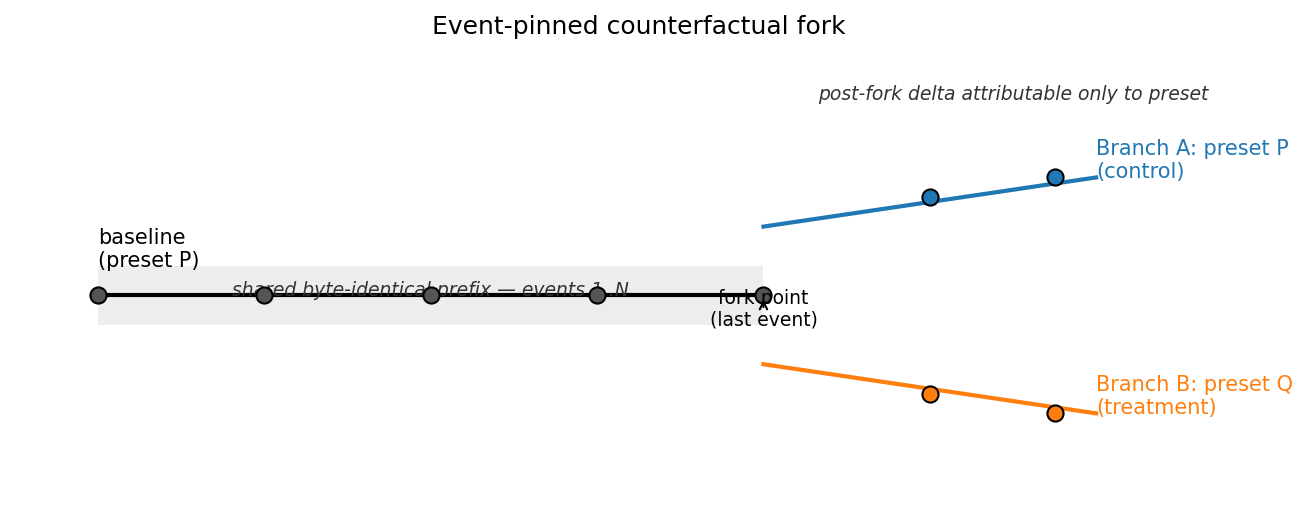
\includegraphics[width=0.88\textwidth]{figures/fig_fork_schematic.png}
  \caption{Event-pinned counterfactual fork 도식. 브랜치는 byte-identical
           prefix를 상속하고 post-fork 설정에서만 발산한다.}
  \label{fig:fork-schematic}
\end{figure}

\textbf{형식적 정의.} nature 세션 $s$는 $(E_s, c_s)$ 쌍으로,
$E_s = (e_1, \ldots, e_n)$은 append-only 이벤트 로그, $c_s$는 해결된
설정 (agent roster, 역할별 모델 override, Pack 설치, prompt
override)이다. 이벤트 로그가 replay의 유일한 source of truth.
fork 연산은
$$
  \mathrm{fork}(s, k, c') \to s', \qquad 1 \le k \le |E_s|,
$$
로, $E_{s'}[1{:}k] = E_s[1{:}k]$ (byte-identical prefix)이고
설정 $c_{s'} = c'$인 새 세션 $s'$를 생성한다; 이후 이벤트
$e_{k+1}^{s'}, e_{k+2}^{s'}, \ldots$는 $c'$ 하에서 생성된다.
연산이 제거하는 두 개 confound: (i) 공유 prefix 위에 정의된 모든
metric은 구성상 $s$와 $s'$에서 동일하며, (ii) 두 sibling
$s_A = \mathrm{fork}(s, k, c_A)$와 $s_B = \mathrm{fork}(s, k, c_B)$의
post-fork metric 차이는 pre-fork stochasticity가 아니라 설정 델타
$c_A \mathbin{\ominus} c_B$에 귀속된다. 잔여 post-fork variance는
fork 지점 이후 발생하는 exogenous/runtime nondeterminism으로
한정된다: LLM 샘플링, tool 호출 부작용, sibling 간 외부 API/파일
상태 drift, aggregator 라우팅 불안정성, runtime 스케줄링 artifact.
연산이 이 잔여 noise를 제거하지는 않으며, 사전-fork prefix를
controlled constant로 격리한다. 페어드 분석에선 같은 $(s, k)$를
$c_A$와 $c_B$로 두 번 fork하여, 공유 prefix에 의한 공분산이 metric
차이의 standard error를 타이트하게 만드는 페어드 관측치를 얻는다
(다음 단락).

\textbf{Fork를 통한 페어드 분석.} 같은 baseline에서 fork된 두 브랜치는
baseline당 페어드 관측치를 제공하므로, metric 차이의 standard error는
페어드 분석에선
$\mathrm{Var}[B-A] = \mathrm{Var}[A] + \mathrm{Var}[B] - 2\,\mathrm{Cov}[A,B]$
이고, 비-페어드에선
$\mathrm{Var}[A]/n_A + \mathrm{Var}[B]/n_B$이다. 공분산 항이 통계적
지렛대이다: baseline 콘텐츠가 두 브랜치의 post-fork 응답에 모두 전달되면
$\mathrm{Cov}[A,B] > 0$가 되어 페어드 CI가 더 타이트해진다. 짧은 코드
분석 followup에서 $N=30$ 페어드 trial로 실증한다
(\texttt{direct-core} baseline $\to$ A=\texttt{direct-core} vs
B=\texttt{haiku-phi4}):

\begin{table}[H]
\centering\small
\begin{tabular}{l r r r}
\toprule
metric & 비-페어드 95\,\% CI halfwidth & 페어드 & ratio \\
\midrule
응답 길이 (chars) & 41.1 & 31.2 & 1.32 \\
Jaccard token overlap & 0.091 (비-페어드 평균) & 0.126 (페어드 평균) & 1.38 ($z=3.19$) \\
\bottomrule
\end{tabular}
\end{table}

두 metric 모두 페어드 타이트닝을 보인다; Jaccard 비율이 약간 더 큼은
content-linked metric이 surface metric보다 더 많은 baseline 공분산을
상속한다는 점과 일관적이다.

\textbf{왜 token Jaccard인가?} Token-set Jaccard는 세 가지 이유로
embedding-cosine 및 exact-match 대안보다 선호되었다. 첫째, 결정적
(deterministic)이며 provider-independent: 버전에 따라 출력이 표류하는
특정 embedding 모델 의존이 없으며, 분석의 재현은 기록된 텍스트와
stop-word 리스트만 있으면 된다. 둘째, $[0,1]$ 범위로 bounded이고
대칭적이라, baseline당 페어드/비-페어드 ratio가 well-formed statistic
이다; 두 브랜치에 모두 등장하는 템플릿 단어는 페어드와 비-페어드
비교에 동일하게 기여하여 cancel되므로 ratio는 그것에 대해 robust.
셋째, 본 논문의 프롬프트들 (open-ended analytical, factual diff,
code summarization)에서 관심사는 paraphrase 동등성이 아니라 두
post-fork 브랜치가 \emph{같은 아키텍처 개념을 명명하는지}
(예: ``EventStore'', ``cascade depth'', ``WebSocket reconnection'')
인데, token overlap이 이를 직접적으로 포착하는 반면 embedding cosine은
공통 concrete 언급이 없어도 fluent paraphrase에 보상한다. 비용은
실재한다: Jaccard는 의미적 동등성을 무시하고 ($x_1$과 $y_1$이
동의어여도 $J(\{x_1\}, \{y_1\}) = 0$) stop-word 리스트에 민감하다.
Semantic-similarity 기반 재현은 자연스러운 향후 확인 작업이다.

\textbf{Regime 조건.} 이 타이트닝은 event-pinned fork의 \emph{보편}
성질이 \emph{아니다}. 세 가지 프롬프트 regime에서 테스트를 확장했다
(각 $n=15$, 동일 A/B 브랜치 구조): P1은 사전 코드 분석에서 ONE concrete
risk를 요구 (\emph{open-ended analytical}); P2는 preset 차이의
런타임 결과 ONE을 요구 (\emph{constrained factual}); P3는 방금
요약한 모듈의 잠재 failure mode ONE을 요구 (\emph{selection with
variety pressure}). P1만이 유의한 페어드 타이트닝을 보인다
(Figure~\ref{fig:paired-regime}):

\begin{table}[H]
\centering\small
\begin{tabular}{l r r r}
\toprule
프롬프트 regime & 페어드 Jaccard & 비-페어드 & ratio ($z$) \\
\midrule
P1 open-ended analytical       & 0.170 & 0.100 & 1.71 ($z=3.41$) \\
P2 constrained factual         & 0.197 & 0.187 & 1.05 ($z=0.70$) \\
P3 selection, variety-sought   & 0.122 & 0.127 & 0.96 ($z=-0.28$) \\
\bottomrule
\end{tabular}
\end{table}

\begin{figure}[H]
  \centering
  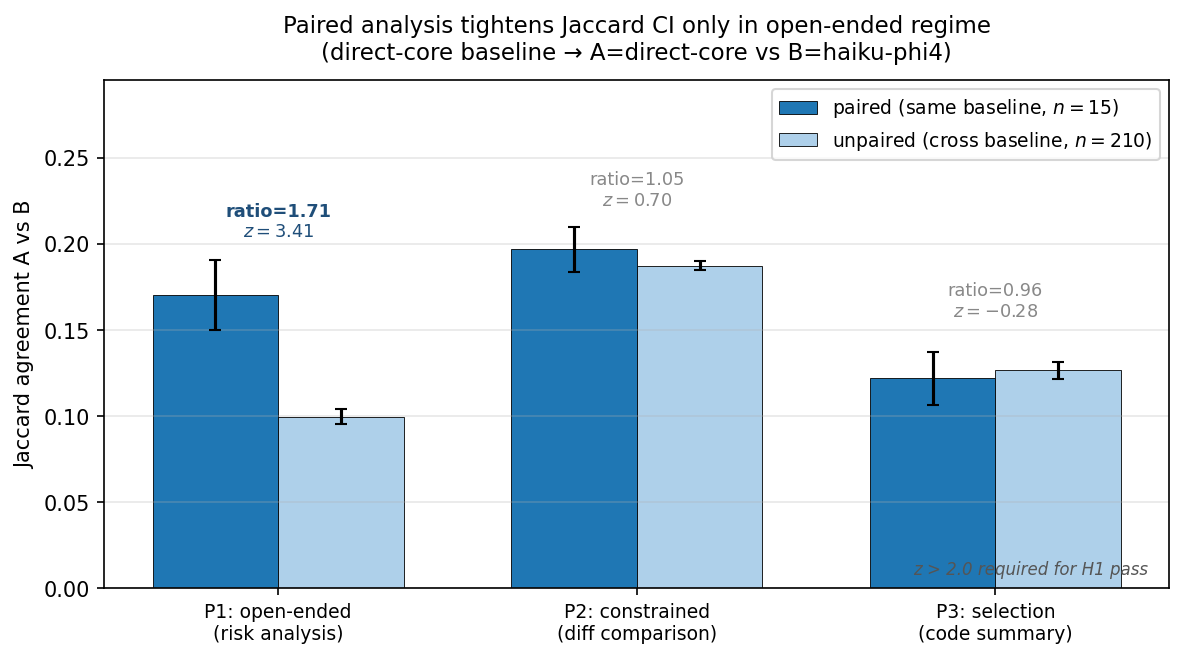
\includegraphics[width=0.88\textwidth]{figures/fig_paired_jaccard_regime.png}
  \caption{세 프롬프트 regime에 걸친 페어드 vs 비-페어드 Jaccard
           (regime당 $n=15$, \texttt{direct-core}$\to$\texttt{haiku-phi4}
           fork). Open-ended analytical regime만 유의한 CI 타이트닝을
           보이며, factual과 selection-with-variety regime은 효과 없음.
           페어드 bar는 same-baseline A--B 일치; 비-페어드 bar는
           cross-baseline 비교를 pool한 것.}
  \label{fig:paired-regime}
\end{figure}

해석: 페어드 분석은 baseline 콘텐츠가 followup 답변 선택을
\emph{steer}할 때 CI를 타이트하게 만든다. 사실 답이 이미 결정되어
있는 프롬프트(P2)나 seed에 걸쳐 다양성이 기대되는 프롬프트(P3)는
이 regime 밖이다. Fork의 페어드 구조를 사용하는 실무자는 commit
이전에 작은 $n$으로 파일럿을 권장한다; CI 감소는 조건부이지 보장이
아니다.

\textbf{수정과 함께 재생.} \texttt{reconstruct()}는 임의의 과거 프레임
트리를 jsonl 로그로부터 재구성한다 \textemdash\ 사후 메트릭 추출, 도구
동작 분석, 아카이브에 대한 프레임워크 수준 변경의 회귀 테스트에 쓰인다.

\textbf{공유 가능 아티팩트.} Pack, Agent, Preset, Host, task, probe
정의는 엄격한 스키마를 갖는 파일 기반이다. 실험과 그 결과는 버전 관리
및 verbatim 공유될 수 있다.

\textbf{Probe.} JSON으로 정의된 단일 축 능력 테스트(계층 T0\textendash T9,
\S\ref{sec:probes}). 한 차원(\texttt{tool.emit},
\texttt{edit.discipline}, \texttt{multi\_turn\_state} 등)을 구조적 성공
기준과 함께 분리. \texttt{nature eval}과 동일 방식으로 Host + Preset과
composable.

\section{사례 연구: preset 수준 벤치마크}
\label{sec:preset-benchmark}

\subsection{설정}

두 이진 설계 축(receptionist vs no-receptionist 토폴로지; cloud-only vs
hybrid downstream 모델 클래스)에 걸친 5개 preset이 cloud / hybrid 설정의
2$\times$2 factorial과 5번째 all-local 설정을 이룬다. 3가지 셋업 타입과
1개 합격 방법(pytest)을 커버하는 5개 태스크에서 실행.

\begin{table}[H]
\centering\small
\begin{tabular}{l c c c c c c c}
\toprule
preset & recep. & core & research. & analyz. & impl. & review. & judge \\
\midrule
\texttt{default}              & H & S & H & S & S & H & H \\
\texttt{direct-core}          & -- & S & H & S & S & H & H \\
\texttt{haiku-phi4}           & H & H & H & P & H & P & P \\
\texttt{direct-haiku-phi4}    & -- & H & H & P & H & P & P \\
\texttt{local-role-optimized} & -- & Q & P & Q & Q & P & P \\
\bottomrule
\end{tabular}
\end{table}

\textit{범례:} H=\texttt{claude-haiku-4-5}, S=\texttt{claude-sonnet-4-6}
(Anthropic API); P=\texttt{phi4:14b}, Q=\texttt{qwen2.5:72b}
(둘 다 Ollama 호스팅, Q4\_K\_M 양자화). ``--''는 해당 역할이 preset
roster에서 빠져있음을 의미 (\texttt{direct-*} preset은 receptionist
계층 없음). 4개 클라우드 preset 내 2.3$\times$ 비용 변동 (passed cell의 preset별 비용 평균 max/min;
(a)~\texttt{direct-core} / \texttt{default}이 core/analyzer/implementer를
Sonnet으로 라우팅하고 (b)~\texttt{haiku-phi4} /
\texttt{direct-haiku-phi4}은 클라우드 역할을 Haiku로 제한하면서
analyzer/reviewer/judge를 로컬 phi4로 오프로딩하기 때문이다.

\textbf{실험 환경.} 하드웨어: Mac Studio, Apple M2 Max, 통합 메모리
96\,GB. 로컬 추론: Ollama 0.20.5, Q4\_K\_M 양자화. 클라우드 추론:
Anthropic direct API (aggregator 없음). 모든 agent는 agent별 기본
temperature 사용; preset 수준 override 없음. nature CLI 0.3.0.
모든 preset/agent JSON 파일과 태스크 정의는 논문의 동반 repository
\url{https://github.com/chanhyeok-made/nature-platform}에 포함.

태스크: \texttt{s1-csv-parser} (small patch, pytest),
\texttt{s3-json-pointer} (small patch, pytest),
\texttt{s4-async-refactor} (medium refactor, pytest),
\texttt{n1-pack-discovery} (medium feature, pytest),
\texttt{x1-pluggy-remove-plugin} (external repo, pytest). 각 셀은 600\,s
세션 watchdog 아래에서 2개 시드로 실행.

\subsection{결과}

\begin{figure}[H]
  \centering
  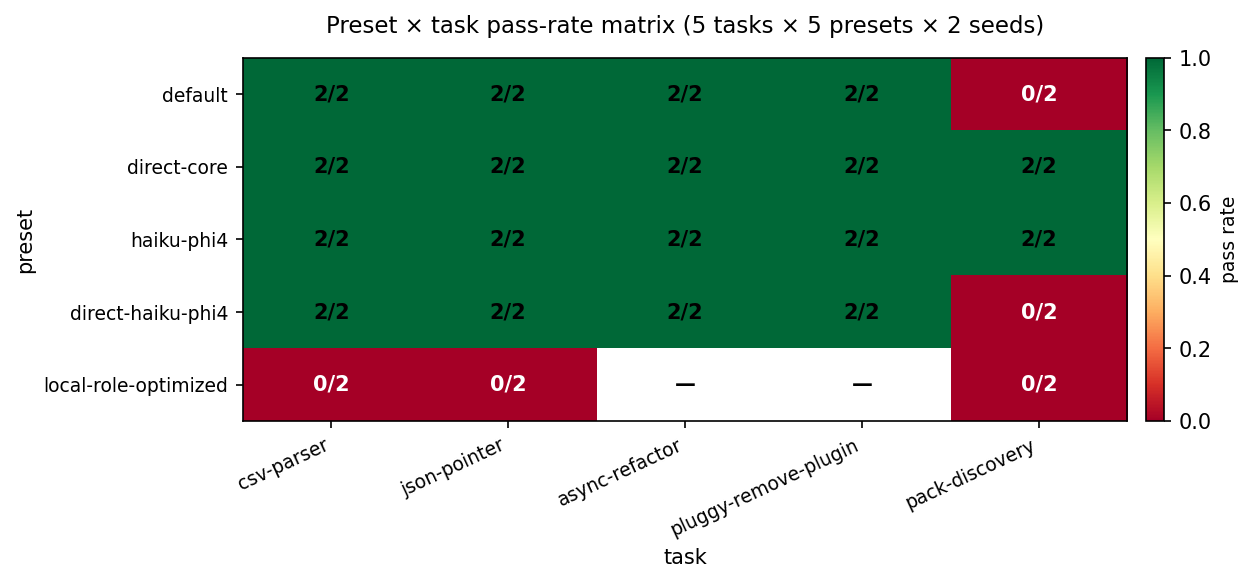
\includegraphics[width=0.95\textwidth]{figures/fig_preset_task_heatmap.png}
  \caption{5개 preset $\times$ 5개 태스크의 합격률 매트릭스. 셀은
           $\{$0, 1, 2$\}$ / 2이며 색이 비율을, 숫자가 $k/n$을 나타낸다.
           \texttt{local-role-optimized}는 3개 태스크에서만 실행되었다
           (모두 0/2).}
  \label{fig:heatmap}
\end{figure}

Figure~\ref{fig:heatmap}이 합격률을 요약한다. 세 가지 발견:

\begin{enumerate}[leftmargin=*,itemsep=2pt,topsep=2pt]
\item \textbf{오직 \texttt{n1-pack-discovery}만이 cloud/hybrid preset들을
      변별한다.} 다른 네 태스크에서는 모든 non-local preset이 두 시드를
      모두 통과한다. \texttt{default} / \texttt{direct-core} /
      \texttt{haiku-phi4} / \texttt{direct-haiku-phi4} 간의 모든
      설정 민감도 신호는 n1에서의 행동 차이로부터 나온다.
\item \textbf{\texttt{local-role-optimized}는 통과하지 않는다.} 6개 셀 중
      5개가 600\,s 타임아웃; 6번째는 acceptance까지 실행됐으나 pytest에서
      실패. 턴 수 6\textendash 17, 도구 에러 수 0\textendash 7
      \textemdash\ 모델이 진전보다 잘못된 도구 인수를 더 자주
      emit하고 있었다.
\item \textbf{다른 4개 preset의 2$\times$2 factorial}
      (Figure~\ref{fig:factorial})은 receptionist 계층이 hybrid에서는
      돕고 (100\,\% vs 80\,\%) pure-haiku에서는 해친다 (80\,\% vs 100\,\%)
      는 점을 시사한다. 관찰된 4개 셀에서 상호작용-일관 교차 경로
      패턴이 보이지만, 셀당 $n=2$가 상호작용 자체에 대한 가설 검정을
      막는다 (\S\ref{sec:limitations}의 sample-size 노트 참조).
      따라서 이는 통계적으로 확립된 효과가 아닌 관찰된 패턴으로
      보고된다.
\end{enumerate}

\begin{figure}[H]
  \centering
  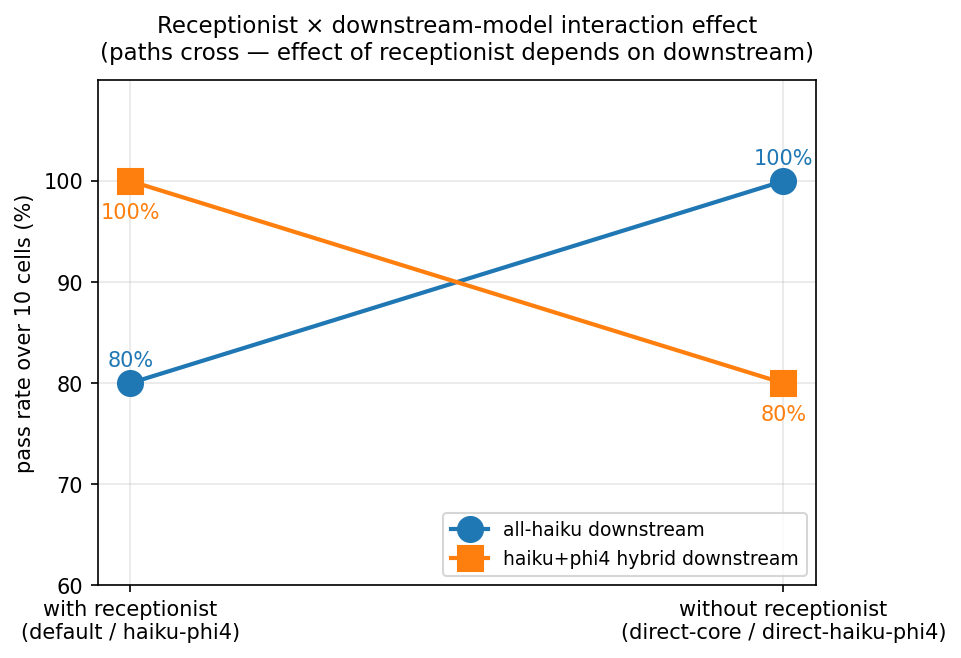
\includegraphics[width=0.75\textwidth]{figures/fig_factorial_interaction.png}
  \caption{Receptionist $\times$ downstream-model 상호작용. Receptionist
           추가는 hybrid downstream을 돕지만 all-haiku downstream을 해친다.}
  \label{fig:factorial}
\end{figure}

\begin{figure}[H]
  \centering
  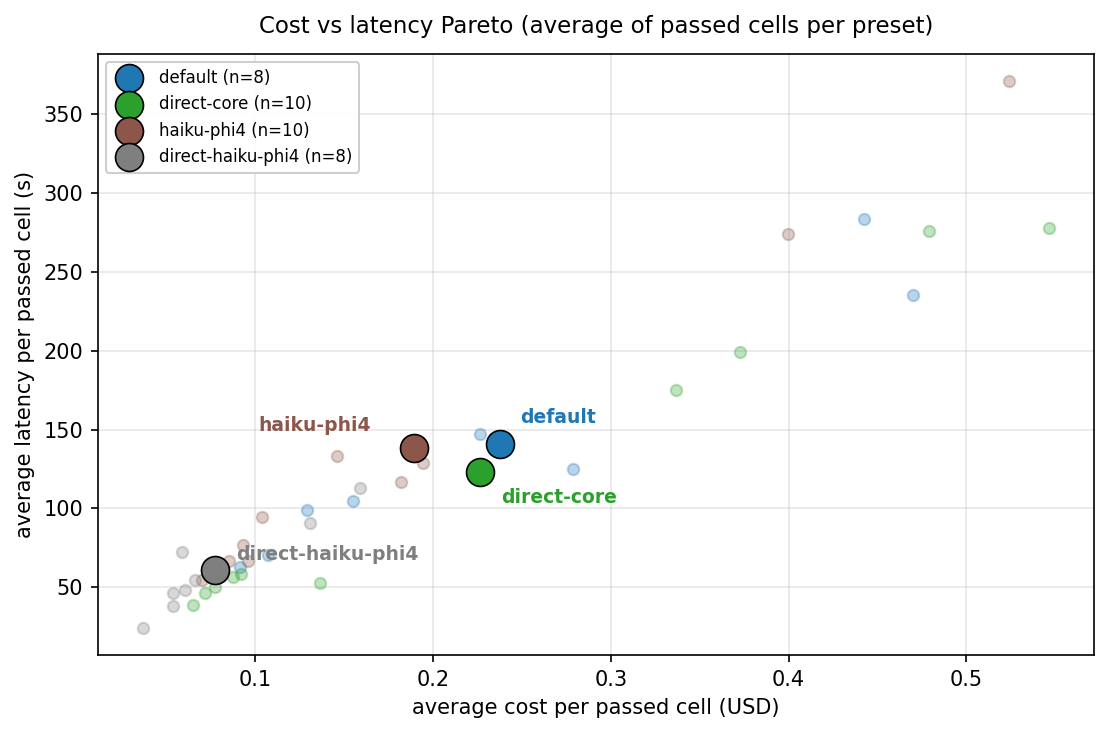
\includegraphics[width=0.85\textwidth]{figures/fig_cost_latency_pareto.png}
  \caption{Preset 간 비용 vs 지연 (합격 셀 평균). \texttt{haiku-phi4}와
           \texttt{direct-core}가 Pareto 경쟁적; \texttt{direct-haiku-phi4}가
           가장 싸고 빠르지만 n1에서 silent failure 위험을 진다.}
  \label{fig:pareto}
\end{figure}

\begin{figure}[H]
  \centering
  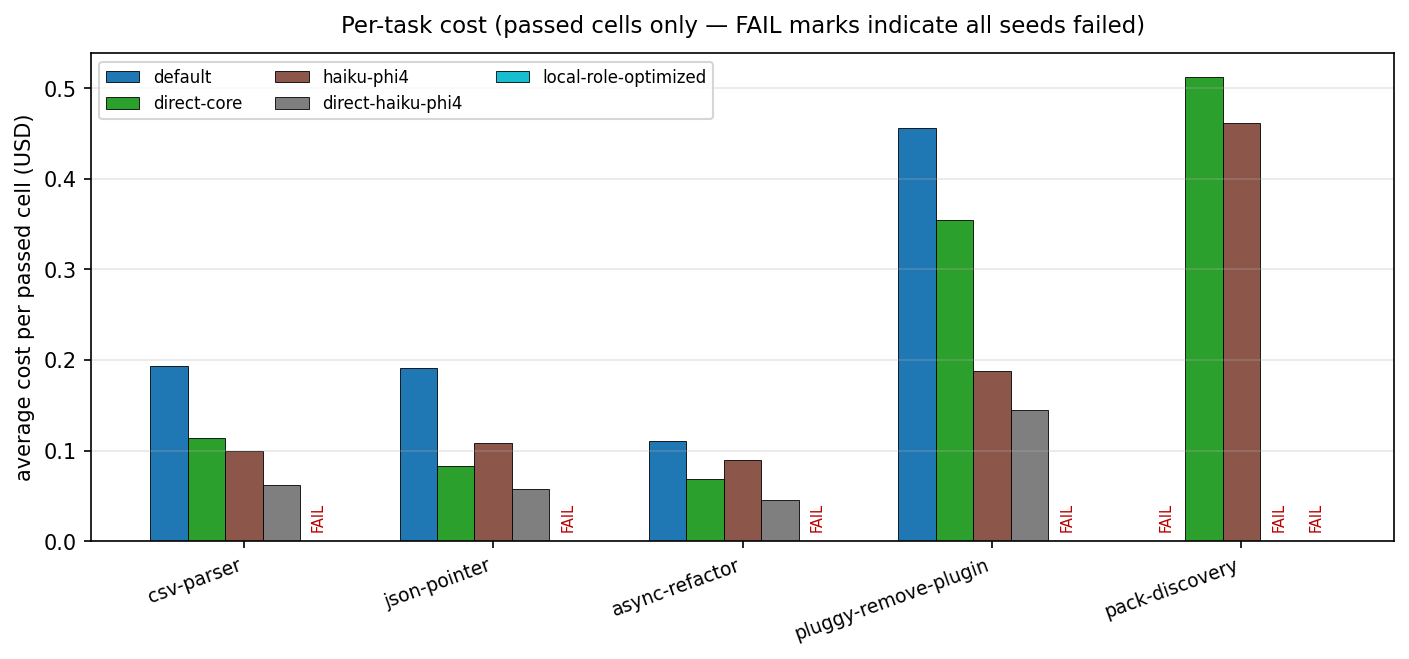
\includegraphics[width=0.95\textwidth]{figures/fig_per_task_cost.png}
  \caption{합격 셀에 대한 태스크별 비용. "FAIL" 마크는 해당 셀의 모든
           시드가 실패했음을 나타낸다.}
  \label{fig:per-task-cost}
\end{figure}

\subsection{관찰된 패턴에 대한 trace 기반 가설}

4개의 실패 n1 셀과 2개의 간신히 통과한 n1 셀에 대한 이벤트 로그 감사는
후보 인과적 이야기를 내놓는다 (검증된 메커니즘이 아니라 trace에 근거한
가설로 제시). n1에서 \texttt{default}는 타임아웃 시점에 평균
91턴, 124 도구 호출, 13 도구 에러를 기록했다 \textemdash\ 세션당
14\textendash 18개 서브프레임을 spawn하며 해결되지 않는 receptionist
$\to$ core $\to$ 4-sub-agent loop. 동일한 n1에서 \texttt{direct-core}는
평균 38턴과 7\textendash 8 서브프레임으로 두 시드 모두 통과했다:
receptionist가 없어 core가 사용자의 원본 프롬프트에서 직접 계획했고
연구자 위임이 더 깨끗했다.

Hybrid에서는 패턴이 뒤집혔다. \texttt{haiku-phi4}는 세션당
12\textendash 15 도구 에러에도 n1을 통과했다 \textemdash\ \emph{\texttt{default}
보다 더 많은 에러} \textemdash\ receptionist 계층이 phi4의 포매팅 실수를
잡는 redundant supervision 역할을 했기 때문이다. Receptionist를 제거한
(\texttt{direct-haiku-phi4})는 더 빠른 완료(173\textendash 248\,s)를
만들었지만 silent \emph{wrong answer}를 냈다: pytest가
\texttt{test\_install\_entry\_can\_reach\_neighbouring\_modules}에서 실패.
Receptionist는 downstream이 강할 때는 프리미엄을 내고 downstream이 약할
때는 배당을 주는 보험 역할을 했다.

\subsection{샘플 크기 주의}

셀당 $n = 2$. 10/10에 대한 Wilson 95\,\% CI는 [72.2\,\%, 100\,\%];
8/10에 대해 [49.0\,\%, 94.3\,\%]. 구간이 겹친다. 가까운 preset 간
합격률 차이에 통계적 유의성을 주장하지 않는다 \textemdash\ 증거는
가설 검정이 아니라 trace 수준(턴 수, 서브프레임 구조, cost-by-agent,
에러 서명)이다. 더 강한 주장을 위해서는 매트릭스에 셀당 5\textendash 10
시드와 더 많은 태스크가 필요하다 (\S\ref{sec:limitations}).

\section{사례 연구: 구성요소 수준 probe}
\label{sec:probes}

Preset 수준 벤치마크는 "어떤 설정이 이 태스크를 완료하는가"에는 답하지만
\emph{왜}는 불투명하게 둔다. 어떤 preset에서 실패하고 다른 preset에서
성공하는 \texttt{(host, model)}은 잘못된 프롬프트, 잘못된 도구, 잘못된
모델 선택, 또는 잠재 인프라 버그를 가질 수 있다. 이를 위해 \emph{probe} suite를
설계했다: 각각 한 축(tool-use, edit-discipline, multi-turn state 등)을
구조적 합격/불합격 기준과 함께 분리하는 32개 계층 등급 능력 테스트.
실행은 결정적이고 재생 가능하다. Probe는 일급 nature 아티팩트이며
\texttt{nature eval}과 동일 방식으로 Host + 모델 계층과 compose된다.
Probe별 상세 논의는 paper repository에 있다; 여기서는 headline 발견을
제시한다.

\subsection{로컬 sweep: Ollama가 호스팅하는 13개 모델}

첫 probe 통과의 모든 모델은 잠재 인프라 버그에 의해 실질적으로 부풀려지거나
축소되었음이 나중에 판명된 점수를 산출했다. 4개 사례
(phi4:14b 3\textendash 25, qwen2.5-coder:32b 4\textendash 21,
llama3.3:70b 3\textendash 22, command-r7b fix 후 변화 없음)가 각각
어댑터/wrapper/타임아웃 스택의 특정 버그에 매핑됐고, 각 수리가 겉보기
모델 랭킹을 이동시켰다. 교훈: \emph{인프라 설정은 측정 변수다}. 실행한
어댑터 스택을 공개하지 않는 벤치마크 보고는 불완전하다.

\subsection{클라우드 sweep: OpenRouter를 통해 라우팅되는 11개 모델}

OpenRouter를 통한 11개 클라우드 모델 $\times$ 32개 probe
(+ 경계 12개 probe를 2개 추가 시드로 재실행) = 총 비용 \$2.56에
$\approx$616 셀. Headline 발견:

\begin{itemize}[leftmargin=*,itemsep=2pt,topsep=2pt]
\item \textbf{Universal long-context ceiling.} \texttt{t3-32k}와
      \texttt{t4-128k}(반복 콘텐츠 위 needle-in-haystack)가 11/11 실패.
      반복 long-context에서 needle 검색은 provider와 세대에 걸쳐 공유된
      현재 클라우드 ceiling이다.
\item \textbf{Provider-family 정성적 특질.} Gemini family (flash + pro)는
      verbatim 지시를 일관되게 paraphrase (\texttt{activeForm} 필드);
      Mixtral 8$\times$22B는 긴 random-looking temp path에서 단일 문자를
      조작; gpt-4o는 paginated Read에서 \texttt{limit=1}을 선택하고 두
      턴 후 파일이 비었다고 선언; llama-3.3-70B는 가장 높은 스키마 준수
      불안정성을 보였다 (3 시드 경계 probe 중 9/12 비일관 통과: 8 flaky
      + 1 consistent-fail). 이것들 중 어느 것도 single-host 측정에서는
      드러나지 않는다.
\item \textbf{측정 변수로서의 플랫폼 friction.} \texttt{qwen-2.5-coder-32b}
      는 OpenRouter 카탈로그에 등재되어 있지만 Cloudflare Workers AI로
      라우팅되며, (a) tool-use 엔드포인트를 advertise하지 않고 (HTTP 404)
      (b) trivial 텍스트 프롬프트에서도 mid-stream 500을 반환한다. 동일
      오픈 웨이트 모델이 로컬 Ollama를 통해서는 정상 작동한다.
\end{itemize}

\subsection{대조}

공유된 29-probe 서브셋에서 10개 클라우드 모델이 25\textendash 29/29에
클러스터링 (10개 모델에 4-point spread); 13개 로컬 모델은
2\textendash 25/29에 걸친다 (23-point spread). Best local
(\texttt{phi4:14b}, \texttt{qwen2.5:72b})이 worst cloud
(OpenRouter 경유 \texttt{llama-3.3-70b})와 25/29에서 만난다. 두 모델이
두 survey에 모두 나타나며; 동일 웨이트의 로컬 q4\_K\_M 대비 클라우드가
29개 중 2\textendash 3 패스를 추가한다 \textemdash\ 더 높은 유효 정밀도
+ 소비자 하드웨어 first-token latency 탈출 덕분.

\textbf{워크플로우 시연과의 연결.} probe 랭킹은
\S\ref{sec:ablations}의 fork 기반 tuning 워크플로우의 경험적
prior 역할을 한다: 특정 역할의 후보들이 그 역할이 운영하는
차원 (예: analyzer/reviewer 역할에 대한 \texttt{tool.emit},
\texttt{edit.discipline}, \texttt{multi\_turn\_state})에서 사전
선별되며, 상위 probe-tier 후보만이 라이브 세션에 fork되어
페어드 검증을 받는다. \texttt{phi4:14b}의 25/29 점수가
\S\ref{sec:ablations}의 model-swap ablation에서 analyzer/reviewer/judge
swap 후보로 선정된 동기이다; fork 프리미티브는 그 probe 수준
역량이 실제 세션의 baseline-consistent post-fork 행동으로
이어지는지 검증한다. \S\ref{sec:probes}의 prior 없이
\S\ref{sec:ablations}는 unscoped 후보 공간을 탐색하게 되었을
것이고, \S\ref{sec:ablations}의 in-session 검증 없이
\S\ref{sec:probes}의 점수는 라우팅 권고로서 untested로 남았을
것이다.

\section{예시 ablation}
\label{sec:ablations}

두 가지 event-pinned ablation이 fork 프리미티브를 보여준다.

\subsection{프롬프트 ablation}

Baseline: 집중된 코드 분석 프롬프트에 대한 \texttt{direct-core} preset.
완료 후(34 이벤트), 세션은 마지막 이벤트에서 fork되어 두 브랜치가 동일한
follow-up 프롬프트를 받았다:

\begin{itemize}[leftmargin=*,itemsep=2pt,topsep=2pt]
\item 브랜치 A (control): 기본 \texttt{researcher.md}(broad 모드)를 가진
      \texttt{direct-core}.
\item 브랜치 B (treatment): 연구자 역할의 지시서 stem을
      \texttt{researcher-scout}로 override한 \texttt{direct-core-scout};
      scout은 \emph{오직} 파일 경로만 반환하고 내용은 반환하지 않는다.
\end{itemize}

두 브랜치는 같은 고수준 아키텍처 리스크(병렬 위임의 concurrency cap
부재)를 식별했다. 브랜치 A의 연구자는 파일 내용을 반환했고; 브랜치 B의
scout은 경로만 반환했으며 core가 경로 의미론 + 구조적 추론으로 리스크를
합성했다. 서브에이전트 프롬프트를 범위 제한해도 caller가 같은 아키텍처
관찰에 도달하는 것을 막지 못했다 \textemdash\ 비용/지연 최적화에 유용한
데이터 포인트이며, swap-and-run 비교는 fresh-run baseline들이 이벤트
1에서부터 발산하기 때문에 정밀하게 만들 수 없는 비교다.

\subsection{모델 스왑 ablation ($n=15$ 시드)}

15개의 독립적인 \texttt{direct-core} baseline을 각각의 마지막 이벤트에서
control 브랜치(\texttt{direct-core})와 treatment 브랜치
(\texttt{haiku-phi4}: analyzer/reviewer/judge가 로컬 phi4:14b로 교체)로
fork. 30개 브랜치 모두 동일한 P1 open-ended followup 수신 (방금 설명한
아키텍처에서 ONE concrete risk 식별, 2\textendash 3 문장). 이것이
\S\ref{sec:primitives}의 fork primitive가 페어드 분석이 효과적인 regime
에서 작동함을 보이는 event-pinned 실증이다; 후보 모델(phi4:14b)은
\S\ref{sec:probes}의 local sweep에서 probe 25/29 pass, local-top tier로
선정되어 analyzer/reviewer/judge 역할에 대한 probe-informed prior이
되었다.

\begin{figure}[H]
  \centering
  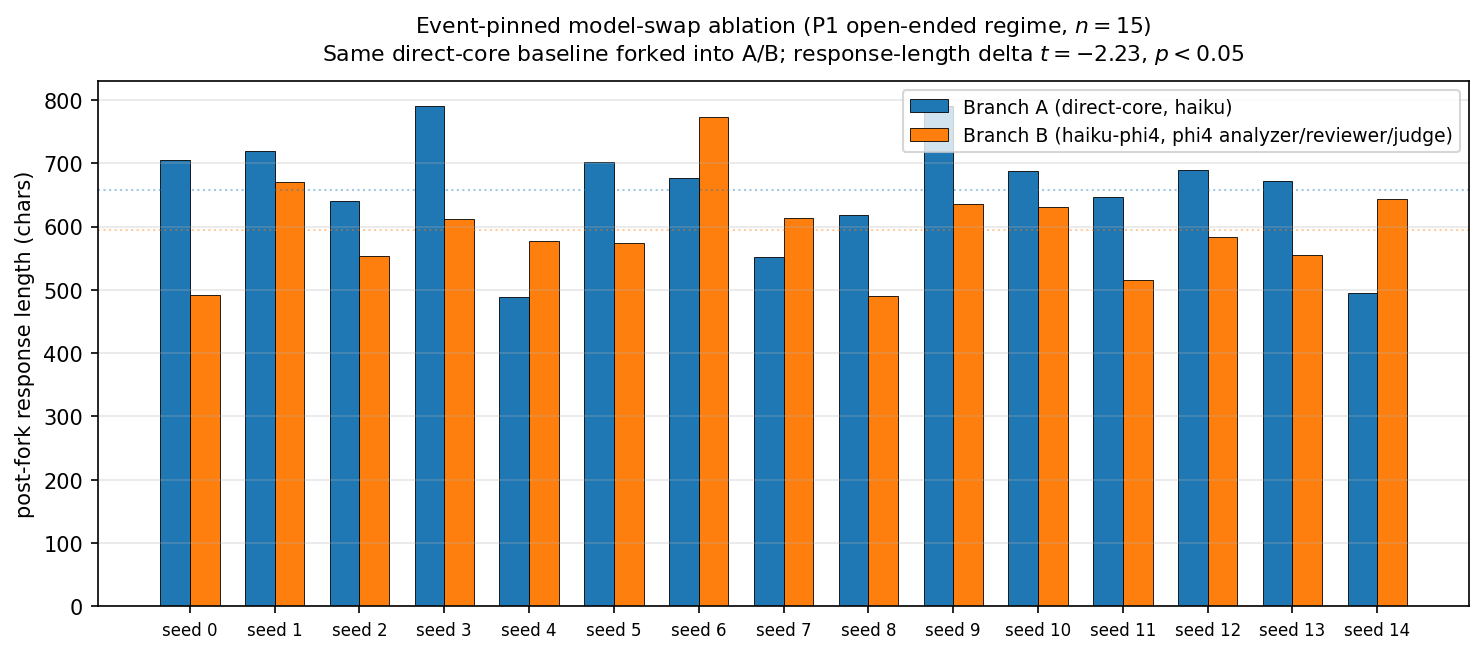
\includegraphics[width=0.92\textwidth]{figures/fig_ablation_model_swap.png}
  \caption{Event-pinned 모델 스왑 ablation ($n=15$ 페어드 시드, P1
           open-ended regime). 각 시드의 \texttt{direct-core} baseline
           이 byte-identical prefix를 공유하는 A(\texttt{direct-core},
           control)와 B(\texttt{haiku-phi4}, treatment) 브랜치로
           fork된다. 평균선 점선 표시. 응답 길이에 대한 페어드
           $t=-2.23$ ($p<0.05$).}
  \label{fig:ablation}
\end{figure}

세 가지 발견:

\begin{itemize}[leftmargin=*,itemsep=2pt,topsep=2pt]
\item \textbf{페어드 Jaccard가 $z=3.41$에서 CI를 타이트하게 만듦.}
      same-baseline A--B token overlap 평균 0.170; cross-baseline 평균
      0.100 (ratio 1.71, Figure~\ref{fig:paired-regime}). Post-fork delta는
      서브에이전트 모델 스왑에 귀속 가능; cross-seed 확률성은 페어링
      으로 통제된다. 이것이 \S\ref{sec:primitives} 프리미티브의 실증적
      payoff다.
\item \textbf{Branch B가 평균 $64 \pm 29$ chars 더 짧게 실행.}
      Phi4 로컬 analyzer/reviewer/judge가 haiku보다 더 간결한 최종
      응답을 생성한다 (페어드 $t=-2.23$, $p<0.05$). \S\ref{sec:primitives}
      의 세 프롬프트 regime에 걸친 부수 측정에서도 verbosity 감소가
      지속된다: P2 $-129 \pm 21$ ch ($t=-6.03$, $p<0.001$), P3
      $-77 \pm 24$ ch ($t=-3.17$, $p<0.01$). 이 $\sim$10\textendash 25\,\%
      간결성은 페어드 Jaccard가 포착한 분석 콘텐츠 일치와 orthogonal
      하며 별도의 실무 관찰이다: 서브에이전트로서의 phi4는 pass/fail
      probe tier와 독립적인 capacity/verbosity 트레이드오프 지점이다.
\item \textbf{수렴과 발산 모두 질적으로 관찰.} 일부 시드에서는 두
      브랜치가 같은 concrete risk로 수렴한다 (예: 시드 0에서 두 브랜치
      모두 \texttt{AreaManager}를 1504-line god object로 식별; 다른 시드들:
      두 브랜치 모두 EventStore를 SPOF로 또는 병렬 도구 race condition
      으로 지목). 다른 시드에서는 관련은 있으나 구별되는 risk에 도달한다.
      페어드 Jaccard가 aggregate 수준에서 이를 포착하며, 어떤 단일 시드도
      단독으로 load-bearing하지 않는다.
\end{itemize}

\S\ref{sec:primitives}의 워크플로우 한 단계로 읽자면: probe 데이터가
phi4:14b를 local-top 후보로 식별; event-pinned fork가 post-fork 방향이
baseline-consistent하게 유지됨을 확인 (페어드 Jaccard 1.71, $z=3.41$);
verbosity가 분석 substance 손실 없이 $\sim$10\,\% 감소. P1-style
워크로드에서 작업하는 실무자는 이 swap을 \emph{accept}할 수 있다.
P2/P3-style 워크로드에 대한 동일 결정은 별도의 fork probe를 요구하는데,
페어드 분석이 그쪽 regime에는 적용되지 않기 때문이다
(\S\ref{sec:primitives}).

\section{논의}
\label{sec:discussion}

\textbf{사례 연구가 주장하지 않는 것.} 세 가지 일반화는 의도적으로
거부한다: 승리 preset 없음 (\S\ref{sec:preset-benchmark}의 태스크 분포에서
일부 설정이 10/10에서 tie를 이루며 다른 분포에서 다르게 랭크될 수 있음),
모델 랭킹 없음 (probe 랭킹은 어댑터 스택에 의존), 통계적 유의성 없음
(셀당 $n = 2$는 합격률 가설 검정에 충분하지 않음). 비교적 주장은 raw
합격률 delta가 아니라 trace 수준 증거에 근거한다.

\textbf{실무자에 대한 시사.} "어떤 모델을 써야 하는가"에서 온 독자는
"내 비용 예산과 지연 tolerance를 감안해 내 태스크 분포 위에서 어떤
\emph{설정}을 쓸까"를 묻고 떠나야 한다. \S\ref{sec:preset-benchmark}의
4개 클라우드 preset은 모두 같은 frontier 모델 family를 사용하며 2.3$\times$
비용과 1.5$\times$ 지연 범위로 (preset별 평균) 80\textendash 100\,\%
합격률을 낸다. 가장
좋은 설정을 고르는 것이 티어 내 모델을 바꾸는 것보다 가치가 크다.

\textbf{연구에 대한 시사.} 파일 기반 아티팩트 (Pack, Preset, Agent, Probe,
task)는 읽기 가능하고, diff 가능하고, git-tractable하다. 새 Probe나
Task는 markdown + JSON 스키마다, 그 이상 없음. 이것은 에이전트
시스템 구성요소의 커뮤니티 기여가 연구 저장소에 벤치마크 태스크를
기여하는 것만큼 lightweight할 수 있는지에 대한 실험이라고 본다.
Event-sourced fork는 prior 시스템에서 찾지 못한 프리미티브이며;
\S\ref{sec:ablations}는 변경 지점이 $t=0$이 아니라 실행 중간에 있을
때 설정 분산 연구의 올바른 도구라고 주장한다.

\section{한계와 향후 연구}
\label{sec:limitations}

\textbf{샘플 크기.} \S\ref{sec:preset-benchmark}는 셀당 $n = 2$의 46개 총
셀 (36 통과, 10 실패); \S\ref{sec:ablations}는 P1 open-ended regime에서
$n=15$ 페어드 시드 (원래 3-시드 파일럿으로부터 업그레이드), 부수적으로
두 개의 추가 regime에서 각각 $n=15$ sweep. \S\ref{sec:primitives}의 페어드
분석 증거 ($N=30$에서 $z=3.19$; $n=15$ P1에서 $z=3.41$)는 페어드 분석이
적용되는 regime 내에서 통계적으로 견고하지만, preset 수준 벤치마크
샘플은 근접 설정 간 합격률 가설 검정에 여전히 underpowered. 5\textendash 10
시드와 15\textendash 20 태스크에서의 follow-up이 preset 매트릭스의 자연스러운
다음 단계로 남는다.

\textbf{페어드 분석 regime 조건.} \S\ref{sec:primitives}의 페어드 CI
타이트닝은 open-ended analytical 프롬프트 regime (P1)에서만 실증되었다.
constrained-factual regime (P2)에서 페어드 비율은 거의 1 (1.05, $z=0.70$);
selection-with-variety regime (P3)에서는 약간 1 이하 (0.96, $z=-0.28$).
따라서 fork가 제공하는 CI 감소는 보편 속성이 아니라 regime 의존 속성이다.
어떤 프롬프트 family가 페어드 분석에서 가장 이득을 보는지 (예: 여기서
관심사인 의미로 답변 공간을 "open-ended"하게 만드는 것이 무엇인지)의
특성화는 향후 연구. 실무자는 페어드 설계에 commit하기 전에 자신의 프롬프트
regime에서 작은 $n$으로 파일럿을 해야 한다.

\textbf{페어드-CI 증거의 통계적 caveat.} \S\ref{sec:primitives}의
페어드-CI 증거에 다음 caveat이 함께 읽혀야 한다. 첫째, $z=3.19$
(Block A)는 $n=870$ 비-페어드 Jaccard 관측치를 독립 sample처럼
취급한다; 실제론 같은 30 baseline의 cross-pairing이라 독립 아니다.
Permutation test가 더 보수적인 (그러나 여전히 유의한) $p$-value를
줄 것이다. 둘째, $N=30$ 심층 실행에 사용된 P1 프롬프트는 실험을
처음 설계할 때 만든 그 프롬프트이므로, 강한 P1 효과는 부분적으로
``analytical 프롬프트''의 unbiased sample이라기보단 selection
artifact이다. 셋째, \S\ref{sec:primitives}의 3-prompt $\times$
3-branch-pair sweep은 9개 페어드/비-페어드 비교로 구성된다;
Bonferroni 보정 시 threshold는 $p<0.0056$이 된다. 헤드라인 P1
결과 ($z=3.41$)는 이 보정을 통과; 더 약한 per-prompt 효과들은
통과하지 못한다. 넷째, 프롬프트-regime 라벨 (open-ended analytical /
constrained factual / selection with variety)은 사후적으로 세
프롬프트를 기술한 것이지, 사전 등록된 카테고리가 아니다.
새 프롬프트 sample에서 사전 등록된 재현이 regime-conditioning
주장을 강화할 것이다.

\textbf{태스크 분포.} pytest로 평가되는 Python 코드 태스크에 편중.
비코드 deliverable 또는 LLM-judge acceptance 태스크는 대표되지 않음.

\textbf{모델 카탈로그.} 11 클라우드 + 13 로컬 모델; 모두 OpenRouter /
Ollama 경유. Anthropic / OpenAI / Google 직접 API는 preset 경로에서
암시적이지만 별도 축으로 비교되지 않음.

\textbf{Cross-framework baseline 없음.} \S2가 LangChain, LlamaIndex,
CrewAI, AutoGen 대비 nature를 positioning하지만 동일 매트릭스를 경쟁
프레임워크로 실행하지 않음. Cross-framework 비교는 별도 논문.

\textbf{Judge-acceptance 검증.} \texttt{s2-docstring-judge}는 LLM-judged
acceptance를 사용하며 judge 자체 동작이 아직 검증되지 않아
\S\ref{sec:preset-benchmark}에서 \emph{제외}됨. 인간 평가 일치 +
adversarial 사례는 별도 연구.

\textbf{Fork helper.} Fork 지점을 가로질러 고아가 된 tool\_use는 다음 LLM
호출에서 API 수준 400을 만든다. \S\ref{sec:ablations}는 baseline의 마지막
이벤트에서 fork하여 이것을 우회했다; 가장 가까운 clean boundary를 고르는
\texttt{--at-resolved-frame} helper가 예정된 작은 follow-up.

\section{결론}

에이전트 시스템 성능은 여러 상호작용하는 선택의 함수다. 설정을 고정하고
모델만 변화시키는 벤치마크는 유용한 한 이야기를 들려준다; 전체 이야기는
아니다. nature의 프리미티브 \textemdash\ 파일 기반 축, event-sourced
실행, counterfactual fork \textemdash\ 는 더 어려운 이야기를 다루기
쉽게 만든다: \emph{설정 분산이 세션 수준에서 모델 분산과 어떻게
상호작용하는가}. 세 사례 연구가 이 프리미티브들이 가능케 하는 것을
보여주고, 샘플 크기가 뒷받침하지 않는 일반화를 명시적으로 거부한다.
플랫폼은 오픈소스다; Pack, Preset, Agent, Probe, task의 기여는 git-tractable
파일로 도착한다. 본 논문의 발견과 발산하는 재현 시도가 가장 정보가
많은 다음 단계로 초대한다.

\bibliographystyle{plain}
\begin{thebibliography}{99}
\bibitem{swebench} Jimenez, C., et al. SWE-bench: Can Language Models Resolve Real-World GitHub Issues? (2023).
\bibitem{agentbench} Liu, X., et al. AgentBench: Evaluating LLMs as Agents. (2023).
\bibitem{humaneval} Chen, M., et al. Evaluating Large Language Models Trained on Code. (2021).
\bibitem{langchain} LangChain. \url{https://python.langchain.com}. (2022\textendash).
\bibitem{crewai} CrewAI. \url{https://www.crewai.com}. (2024\textendash).
\bibitem{autogen} Wu, Q., et al. AutoGen: Enabling Next-Gen LLM Applications. Microsoft Research (2023).
\bibitem{mcp} Model Context Protocol specification. \url{https://modelcontextprotocol.io}. (2024\textendash).
\bibitem{fowler-es} Fowler, M. Event Sourcing. \url{https://martinfowler.com/eaaDev/EventSourcing.html}. (2005).
\bibitem{anthropic-toolcall} Anthropic. Tool Use with Claude. Technical documentation (2024).
\bibitem{mlflow} Zaharia, M., et al. Accelerating the Machine Learning Lifecycle with MLflow. IEEE Data Eng Bull (2018).
\bibitem{wandb} Weights \& Biases. \url{https://wandb.ai}. (2017\textendash).
\bibitem{langgraph} LangGraph. State graph orchestration with checkpointing. \url{https://langchain-ai.github.io/langgraph/}. (2024\textendash).
\bibitem{langsmith} LangSmith. Trace, evaluate, and monitor LLM applications. \url{https://docs.smith.langchain.com/}. (2023\textendash).
\bibitem{llamaindex} LlamaIndex. Data framework for LLM applications. \url{https://docs.llamaindex.ai/}. (2023\textendash).
\end{thebibliography}

\end{document}
